\documentclass[11pt,letterpaper]{article}
\usepackage[margin=1in]{geometry}
\usepackage[T1]{fontenc}
\usepackage[utf8]{inputenc}
\usepackage{lmodern,microtype}
\usepackage{amsmath,amssymb,amsthm,mathtools}
\usepackage{booktabs,tabularx,array}
\usepackage{graphicx,xcolor,tikz,pgfplots}
\usetikzlibrary{arrows.meta,positioning,calc,fit,backgrounds,shapes.geometric}
\pgfplotsset{compat=1.18}
\usepackage{caption}
\usepackage[colorlinks=true,linkcolor=blue!45!black,citecolor=blue!45!black,urlcolor=blue!45!black]{hyperref}
\hypersetup{pdftitle={Relational Interfaces, Subspaces, and Operator-Valued Coupling in Gauge-VFE Attention}}
\newcommand{\R}{\mathbb R}
\newcommand{\KL}{D_{\mathrm{KL}}}
\newcommand{\SPD}{\operatorname{SPD}}
\newcommand{\GL}{\operatorname{GL}}
\newcommand{\SO}{\operatorname{SO}}
\newcommand{\tr}{\operatorname{tr}}
\newcommand{\rank}{\operatorname{rank}}
\newcommand{\im}{\operatorname{im}}
\newcommand{\softmax}{\operatorname{softmax}}
\newcommand{\diag}{\operatorname{diag}}
\newcommand{\E}{\mathbb E}
\newcommand{\Cov}{\operatorname{Cov}}
\newcommand{\svec}{\operatorname{svec}}
\newcommand{\dd}{\mathop{}\mathrm{d}}
\newtheorem{proposition}{Proposition}[section]
\newtheorem{corollary}[proposition]{Corollary}
\theoremstyle{remark}
\newtheorem{remark}[proposition]{Remark}
\definecolor{receive}{RGB}{0,114,178}
\definecolor{send}{RGB}{213,94,0}
\definecolor{content}{RGB}{0,135,108}
\definecolor{violet}{RGB}{125,80,160}
\tikzset{
 box/.style={draw,rounded corners,minimum height=10mm,text width=29mm,align=center,fill=black!2},
 arr/.style={-{Stealth[length=2mm]},thick},
 every node/.style={font=\small}
}
\setlength{\emergencystretch}{2em}
\setlength{\parskip}{0.3em}
\setcounter{tocdepth}{2}
\title{Relational Interfaces, Subspaces, and\\ Operator-Valued Coupling in Gauge-VFE Attention}
\author{Technical synthesis and exploratory constructions\\Gauge--VFE research program}
\date{September 13, 2026}
\begin{document}
\maketitle
\begin{abstract}
This note develops a discussion about whether the query, key, and value roles of attention require separate agent frames, separate pairwise interfaces, or different operators within one frame. We distinguish directions of interaction from relevance, content, and state update; frame changes from physical endomorphisms; and invertible transport from subspace selection. The Gaussian attention energy is expanded in full before specializing to separate sending and receiving frames and to special-orthogonal transport. Frame-dependent projectors and reduced-coordinate marginals can select overlapping aspects of a shared belief without assigning fixed cognitive faculties to coordinates. We distinguish mixture prediction from precision pooling and construct conditional source/content models in which a value can differ from a key without a third physical frame. Existing program derivations are attributed, and proposed extensions are labeled as model choices. Small examples and algebra checks accompany the derivations. Saved single-seed QKV ablations motivate controlled experiments without establishing a performance mechanism. No result proves parity with a vanilla transformer or removes the need to specify a learning objective.
\end{abstract}
\begin{center}
\small Research note: exact identities, conditional constructions, and open empirical questions. Full-input routing, independent query/key frames, and selectable ablations are implemented; their performance hypotheses remain untested.
\end{center}
\tableofcontents
\clearpage

\section{The question and the existing research}
The discussion began with an empirical observation: learned key and value maps improved a small gauge-VFE language model in the available runs, while adding a query map produced little additional benefit. It then moved to the meaning of the three roles. Must receiving, sending, and transmitted content have different frames, or can they be different operations on one underlying belief? The mathematical issue is whether relevance, content, and response must use the same full-space operator. Words such as hearing and speaking can suggest roles, but do not supply the mathematics.

Several alternatives emerged. One frame per agent supplies relative transport to every partner. Two role frames distinguish receiving and sending while remaining shared across partners. Partner-specific endpoint frames remove much of the compatibility imposed by shared vertex frames. A third value frame adds algebraic freedom but does not follow from counting communication directions. Finally, one common frame with overlapping subspaces or readout operators can distinguish roles without assigning permanent cognitive labels to coordinates.

This note develops these alternatives. Two directions of influence do not imply two scalar variables, and three attention factors do not imply three physical directions. A matrix is not a subspace; an invertible change of coordinates is not an information-losing projection; an exact dot-product cross term is not an equivalence of complete attention dynamics.

\subsection{Continuity and status}
The live \emph{GL(K) attention} manuscript, Sections \texttt{sec:untied\_qk} and \texttt{sec:value\_aggregation}, already derives Gaussian query/key factors and transported mixture means. The live \emph{Gauge-VFE transformer correspondence} manuscript gives the factor-pair characterization C1, full sufficient-statistic representation C2, normalized source/content model C3, gradient obstruction C5, and precision/mixture distinctions C7--C9. The live \emph{PIFB2} manuscript, \texttt{sec:transport} and \texttt{sec:discrete\_regime\_ii}, distinguishes flat vertex transport from independent links. The repository's receiver-quotient design already defines reduced-coordinate Gaussian comparison. These are existing constructions, not discoveries of this note.

The synthesis concerns their relationships and the remaining choices: which maps are coordinates and which are physical responses, how subspace selection transforms, when projected comparison defines quotient transport, and what objective learns useful content. The accompanying source manifest identifies the inspected revisions. Manuscripts are works in progress; the hypotheses and derivations below determine each claim's scope.

An \emph{exact identity} is algebra within stated domains. A \emph{conditional construction} defines a model and derives its consequences without claiming that the original theory forces that model. An \emph{empirical observation} reports saved artifacts. A \emph{hypothesis} requires a controlled experiment. Numerical checks illustrate formulas rather than prove universal statements.

We use finite-dimensional real Gaussian beliefs and finite nonempty attention supports. Covariances are positive definite unless a reduced coordinate space is explicitly introduced. Exact full-Gaussian identities do not automatically survive diagonal approximation, clipping, frozen derivatives, or a changed objective. An agent here is a subsystem or token occurrence; no cognitive or physical interpretation is asserted.

\section{Two directions, three roles, and an operator}
\label{sec:directions}
For two classical subsystems, a schematic interaction is
\begin{equation}
 \dot x_i=f_i(x_i)+I_{i\leftarrow j}(x_i,x_j),\qquad
 \dot x_j=f_j(x_j)+I_{j\leftarrow i}(x_j,x_i).
 \label{eq:two-directions}
\end{equation}
There are two endpoint directions. Either interaction may vanish, and a common potential may constrain them, but each can have many components. This local ODE schematic does not assert that all field or quantum interactions close on two marginal subsystem states. A joint quantum state can carry correlations absent from its marginals.

Advanced and retarded Green functions distinguish temporal support and boundary conditions. They do not merely rename the endpoint directions in \eqref{eq:two-directions}. Wheeler--Feynman absorber theory and Cramer's transactional interpretation give specific time-symmetric constructions, not a proof that all interactions require two frames or that queries and keys are advanced and retarded waves \cite{WheelerFeynman1945,Cramer1986}. The useful analogy is simply that an interaction depends on both endpoints.

\subsection{Vanilla attention}
With column vectors, one attention head is
\begin{align}
 Q_i&=W_Qx_i,\qquad K_j=W_Kx_j,\qquad V_j=W_Vx_j,\\
 a_{ij}&=\softmax_{j\in\mathcal J_i}
 \left(\frac{Q_i^\top K_j}{\sqrt{k}}+b_{ij}\right),\\
 y_i&=W_O\sum_{j\in\mathcal J_i}a_{ij}V_j.
 \label{eq:vanilla}
\end{align}
The matrices are shared across positions in the head and layer. A query is reused against the permitted keys; it is not recomputed separately for each partner in that operation. Earlier computation can make $x_i$ contextual, and different partners give different scores \cite{Vaswani2017}.

Matching and transmitted output have composites
\begin{equation}
 M=W_Q^\top W_K,\qquad C=W_OW_V.
\end{equation}
For invertible $S,T$ of the respective head dimensions, the changes
\begin{equation}
 (W_Q,W_K)\mapsto(SW_Q,S^{-\top}W_K),\qquad
 (W_V,W_O)\mapsto(TW_V,W_OT^{-1})
\end{equation}
preserve these composites. This parameter redundancy alone is not a local physical gauge theory.

Both $Q_i$ and $K_j$ participate in $j\to i$. The reverse direction uses $Q_j$ and $K_i$. A value is content on an existing direction. Query, key, and value are computational roles rather than three cognitive compartments.

\begin{figure}[tb]
\centering
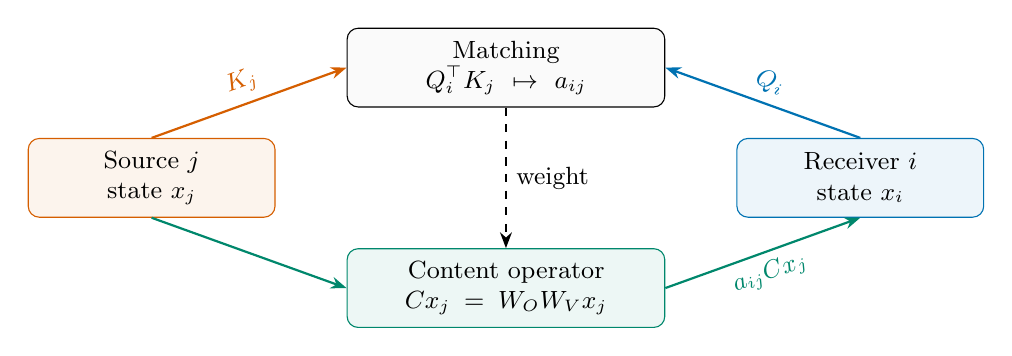
\begin{tikzpicture}
\node[box,draw=send,fill=send!7] (src) at (0,0) {Source $j$\\state $x_j$};
\node[box,draw=receive,fill=receive!7] (dst) at (9,0) {Receiver $i$\\state $x_i$};
\node[box,text width=38mm] (match) at (4.5,1.4) {Matching\\$Q_i^\top K_j\mapsto a_{ij}$};
\node[box,text width=38mm,draw=content,fill=content!7] (msg) at (4.5,-1.4) {Content operator\\$Cx_j=W_OW_Vx_j$};
\draw[arr,send] (src.north) -- node[above,sloped] {$K_j$} (match.west);
\draw[arr,receive] (dst.north) -- node[above,sloped] {$Q_i$} (match.east);
\draw[arr,content] (src.south) -- (msg.west);
\draw[arr,content] (msg.east) -- node[below,sloped] {$a_{ij}Cx_j$} (dst.south);
\draw[arr,dashed] (match.south) -- node[right] {weight} (msg.north);
\end{tikzpicture}
\caption{\textbf{One directed contribution, two operations.} Query and key determine relevance; the content operator determines the transmitted vector. The reverse direction has its own receiver/source assignment.}
\end{figure}

\subsection{Operator-valued coupling}
An aggregation
\begin{equation}
 m_i=\sum_j\beta_{ij}\Omega_{ij}\mu_j,\qquad
 \mathcal C_{ij}=\beta_{ij}\Omega_{ij},
 \label{eq:coupling}
\end{equation}
already includes a value-like operation. The scalar controls strength, the matrix determines how source components enter receiver coordinates, and $\mathcal C_{ij}\mu_j$ is the contribution. If $\beta_{ij}>0$ and $\Omega_{ij}$ is invertible, $\mathcal C_{ij}$ has full rank. This does not imply equal treatment of directions: a full-rank general-linear operator can be highly anisotropic. A masked zero-weight edge is an exception.

An independent value map adds content freedom at fixed matching. Its absence does not mean \eqref{eq:coupling} transmits no values. Conversely, an arbitrary content map cannot generally be absorbed into invertible transport while preserving compatibility and covariance transformations.

\section{One frame per agent and its constraints}
\label{sec:oneframe}
Let $E_i\simeq\R^d$ be a local belief space and $U_i:F\to E_i$ an invertible frame from a reference space. Write
\begin{equation}
 q_i=\mathcal N(\mu_i,\Sigma_i),\qquad \Sigma_i\in\SPD(d).
\end{equation}
A passive coordinate change $g_i$ acts as
\begin{equation}
 \mu_i'=g_i\mu_i,\quad \Sigma_i'=g_i\Sigma_i g_i^\top,\quad U_i'=g_iU_i.
 \label{eq:gauge}
\end{equation}
Other maps and metrics must transform consistently. Passive covariance does not imply that actively changing a learned frame with a fixed observation model preserves predictions.

Vertex transport is
\begin{equation}
 \Omega_{ij}=U_iU_j^{-1},\qquad \Omega_{ij}'=g_i\Omega_{ij}g_j^{-1}.
 \label{eq:flat}
\end{equation}
One frame per vertex already yields pair-dependent transports. It imposes
\begin{equation}
 \Omega_{ii}=I,\quad \Omega_{ij}\Omega_{jk}=\Omega_{ik},\quad
 \Omega_{ji}=\Omega_{ij}^{-1},\quad \Omega_{ij}\Omega_{jk}\Omega_{ki}=I.
\end{equation}
Adjacent inverse factors cancel. The restriction is cross-pair compatibility, not absence of partner dependence.

Independent edge factors give
\begin{equation}
 \Omega_{ij}=U_iL_{ij}U_j^{-1},\qquad
 H_{ijk}=U_i(L_{ij}L_{jk}L_{ki})U_i^{-1}.
 \label{eq:edge}
\end{equation}
A nonidentity link does not guarantee a nonidentity loop product. For a connection whose opposite orientation is reverse traversal of the same edge, require $L_{ji}=L_{ij}^{-1}$. Independently directed communication channels need not satisfy this condition.

The property $H\ne I$ is conjugation invariant, whereas $\|H-I\|_F$ is not generally invariant under $\GL(d)$ conjugation. Trace and eigenvalues give some invariants, but can miss a nonidentity unipotent matrix. Edge transport in gauge-equivariant learning obeys endpoint covariance \cite{deHaan2021,Weiler2021}; this does not identify every learned pairwise matrix with a physical field.

\begin{figure}[tb]
\centering
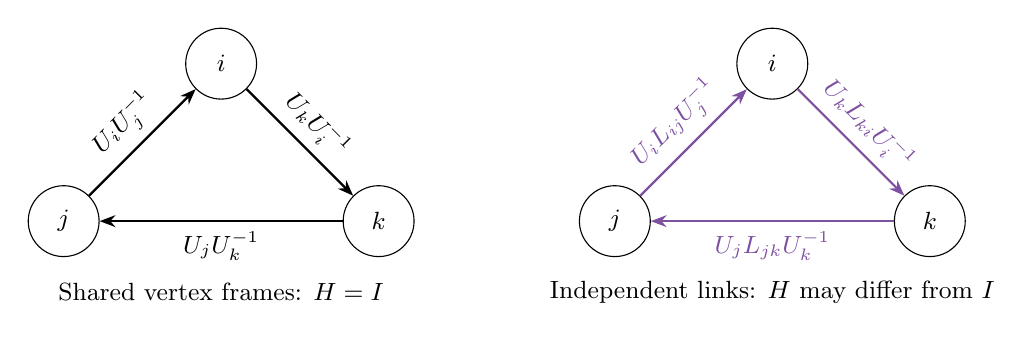
\begin{tikzpicture}
\node[circle,draw,minimum size=9mm] (i) at (0,2) {$i$};
\node[circle,draw,minimum size=9mm] (j) at (-2,0) {$j$};
\node[circle,draw,minimum size=9mm] (k) at (2,0) {$k$};
\draw[arr] (j) -- node[above,sloped] {$U_iU_j^{-1}$} (i);
\draw[arr] (k) -- node[below] {$U_jU_k^{-1}$} (j);
\draw[arr] (i) -- node[above,sloped] {$U_kU_i^{-1}$} (k);
\node at (0,-0.9) {Shared vertex frames: $H=I$};
\node[circle,draw,minimum size=9mm] (ii) at (7,2) {$i$};
\node[circle,draw,minimum size=9mm] (jj) at (5,0) {$j$};
\node[circle,draw,minimum size=9mm] (kk) at (9,0) {$k$};
\draw[arr,violet] (jj) -- node[above,sloped] {$U_iL_{ij}U_j^{-1}$} (ii);
\draw[arr,violet] (kk) -- node[below] {$U_jL_{jk}U_k^{-1}$} (jj);
\draw[arr,violet] (ii) -- node[above,sloped] {$U_kL_{ki}U_i^{-1}$} (kk);
\node at (7,-0.9) {Independent links: $H$ may differ from $I$};
\end{tikzpicture}
\caption{\textbf{Partner dependence and independent geometry.} Both constructions give pair-dependent transport. The right-hand construction releases the vertex cocycle constraint.}
\end{figure}

\section{The full Gaussian attention energy}
\label{sec:gaussian}
Let $S_{ij}=\Omega_{ij}\Sigma_j\Omega_{ij}^\top$. The exact transported divergence is
\begin{equation}
 D_{ij}=\frac12\left[
 \log\frac{\det S_{ij}}{\det\Sigma_i}-d+\tr(S_{ij}^{-1}\Sigma_i)
 +(\mu_i-\Omega_{ij}\mu_j)^\top S_{ij}^{-1}(\mu_i-\Omega_{ij}\mu_j)
 \right].
 \label{eq:gausskl}
\end{equation}
It is invariant under \eqref{eq:gauge}: trace and quadratic factors cancel, as do the two determinant Jacobians. This is the Gaussian instance of relative-entropy invariance under a common invertible pushforward \cite{KullbackLeibler1951}. It requires transporting the full distribution.

\subsection{Entropy-regularized source selection}
For finite energies on a nonempty support $\mathcal J_i$, positive normalized $\pi_{ij}$, and $\tau>0$, minimize
\begin{equation}
 \mathcal F_i(\beta)=\sum_j\beta_{ij}D_{ij}
 +\tau\sum_j\beta_{ij}\log\frac{\beta_{ij}}{\pi_{ij}},
 \qquad \beta_i\in\Delta(\mathcal J_i).
 \label{eq:cat}
\end{equation}
Stationarity with a normalization multiplier gives
$D_{ij}+\tau[\log(\beta_{ij}/\pi_{ij})+1]+\lambda_i=0$.
Strict convexity yields the unique solution
\begin{equation}
 \boxed{\beta_{ij}=\frac{\pi_{ij}e^{-D_{ij}/\tau}}
 {\sum_\ell\pi_{i\ell}e^{-D_{i\ell}/\tau}}.}
 \label{eq:softmax}
\end{equation}
This is exact source selection for \eqref{eq:cat}. Arbitrary temperature does not automatically produce an ordinary ELBO for an unchanged likelihood; powered densities require their own normalizers.

\subsection{The cross term and its restrictions}
Under flat transport define
\begin{equation}
 \xi_i=U_i^{-1}\mu_i,\quad C_i=U_i^{-1}\Sigma_iU_i^{-\top},\quad
 H_i=C_i^{-1},\quad S_i=C_i+\xi_i\xi_i^\top.
\end{equation}
Then
\begin{equation}
 D_{ij}=\frac12\left[
 \log\det C_j-\log\det C_i-d+\tr(H_jS_i)
 -2\xi_i^\top H_j\xi_j+\xi_j^\top H_j\xi_j\right].
 \label{eq:canonical-kl}
\end{equation}
In physical coordinates the cross term is
\begin{equation}
 \boxed{\mu_i^\top\Omega_{ij}^{-\top}\Sigma_j^{-1}\mu_j
 =(U_i^{-1}\mu_i)^\top(U_j^\top\Sigma_j^{-1}\mu_j).}
 \label{eq:qk}
\end{equation}
Thus $Q_i=U_i^{-1}\mu_i$ and $K_j=U_j^\top\Sigma_j^{-1}\mu_j$. Matrix order matters.

These factors are constrained. If $A=U^{-1}$ and $B=U^\top\Sigma^{-1}$, then $A^\top B=\Sigma^{-1}\succ0$. Conversely, invertible $A$ with $A^\top B\succ0$ admits $U=A^{-1}$ and $\Sigma=(A^\top B)^{-1}$. This reconstructs C1 of the correspondence manuscript. The pair $A=I$, $B=\diag(1,-1)$ is excluded. Different query/key formulas do not confer arbitrary independent factors.

The full score also factors in sufficient statistics. Choose $\svec$ so that $\svec(A)^\top\svec(B)=\tr(AB)$ for symmetric matrices, and set
\begin{align}
 \mathsf q_i&=(\xi_i,\svec(S_i),1),\\
 \mathsf k_j&=\left(H_j\xi_j,-\tfrac12\svec(H_j),
 -\tfrac12[\xi_j^\top H_j\xi_j+\log\det C_j]\right).
\end{align}
Equation \eqref{eq:canonical-kl} gives
\begin{equation}
 -D_{ij}=\mathsf q_i^\top\mathsf k_j+\tfrac12(\log\det C_i+d).
 \label{eq:lift}
\end{equation}
The last term cancels within a row softmax. This recovers C2: the full score is an exact dot product in dimension $d+d(d+1)/2+1$, with constrained nonlinear sufficient statistics and temperature $1/\tau$. Pair-specific links or receiver-specific marginals do not automatically have this global factorization.

\section{Separate sending and receiving frames}
\label{sec:twoframes}
Let $A_i,B_i$ be invertible role maps and define
\begin{equation}
 \Omega_{ij}=A_iB_j^{-1}.
\end{equation}
For now they act between declared belief coordinates. The distinction between physical operators and coordinate copies is made below. Set
\begin{equation}
 x_i=A_i^{-1}\mu_i,\quad P_i=A_i^{-1}\Sigma_iA_i^{-\top},\quad
 H_j=B_j^\top\Sigma_j^{-1}B_j,\quad k_j=B_j^\top\Sigma_j^{-1}\mu_j,
\end{equation}
and $r_j=\mu_j^\top\Sigma_j^{-1}\mu_j$. Here $P_i$ is a covariance; later projectors use $\mathsf P_i$.

\begin{proposition}[Two-frame decomposition]
The exact divergence is
\begin{align}
 D_{ij}=\frac12\big[&
 \log\det\Sigma_j-\log\det\Sigma_i
 +2\log|\det A_i|-2\log|\det B_j|-d \nonumber\\
 &+\tr(H_jP_i)+x_i^\top H_jx_i-2x_i^\top k_j+r_j\big].
 \label{eq:two-kl}
\end{align}
\end{proposition}
\begin{proof}
The transported precision is
$A_i^{-\top}B_j^\top\Sigma_j^{-1}B_jA_i^{-1}$.
Its trace against $\Sigma_i$ is $\tr(H_jP_i)$. Expanding the mean quadratic gives $x_i^\top H_jx_i-2x_i^\top k_j+r_j$. The transported determinant is $\det\Sigma_j(\det A_i)^2/(\det B_j)^2$. Substitution proves the formula.
\end{proof}
Removing only row-constant terms gives
\begin{align}
 \beta_{ij}=\softmax_j\bigg[
 &\frac{x_i^\top k_j}{\tau}+\log\pi_{ij}\nonumber\\
 &-\frac{x_i^\top H_jx_i+\tr(H_jP_i)+r_j
 +\log\det\Sigma_j-2\log|\det B_j|}{2\tau}\bigg].
\end{align}
Separate role frames release the one-frame factor-pair constraint, but retain uncertainty corrections and square invertibility. Exponential parameterizations add their own range restrictions. No performance claim follows.

\subsection{Special-orthogonal reduction}
\label{sec:so}
Take $A_i=R_{Qi}$, $B_j=R_{Kj}\in\SO(d)$ and common covariance $\Sigma_i=\sigma^2I$. Transport preserves covariance, so
\begin{align}
 D_{ij}&=\frac{\|\mu_i-R_{Qi}R_{Kj}^\top\mu_j\|^2}{2\sigma^2}
 =\frac{\|Q_i-K_j\|^2}{2\sigma^2},\\
 Q_i&=R_{Qi}^\top\mu_i,\qquad K_j=R_{Kj}^\top\mu_j.
\end{align}
Therefore
\begin{equation}
 \boxed{\beta_{ij}=\softmax_j\left[
 \frac{Q_i^\top K_j}{\tau\sigma^2}
 -\frac{\|K_j\|^2}{2\tau\sigma^2}+\log\pi_{ij}\right].}
 \label{eq:so}
\end{equation}
Equal key norms on the allowed support remove the second term. With $\tau\sigma^2=\sqrt d$, the vanilla weight formula with prior bias is recovered. Rotations do not enforce equal norms across tokens: $\|Q_i\|=\|K_i\|=\|\mu_i\|$. At fixed $\mu_i$, directions can vary independently but lengths cannot.

Anisotropic covariances retain mismatch terms even for rotations. Unequal isotropic variances retain trace and log-ratio terms and a source-dependent variance denominator. Both the group and common-isotropy assumptions are needed.

Using the same map for mixture content gives
\begin{equation}
 \sum_j\beta_{ij}\Omega_{ij}\mu_j
 =R_{Qi}\sum_j\beta_{ij}K_j.
 \label{eq:so-value}
\end{equation}
Keys and values are tied in role-reference coordinates, followed by the receiving rotation.

\subsection{Role bridges and composition}
\label{sec:bridges}
Two readings are consistent but different. If both role maps land in the same physical $E_i$, identity handoff at an intermediate vertex gives
\begin{equation}
 \Omega_{ij}\Omega_{jk}=A_i(B_j^{-1}A_j)B_k^{-1}.
\end{equation}
The reference-space endomorphism $D_j=B_j^{-1}A_j$ represents additional response structure. Choosing $U_j=B_j$ makes its physical representative $U_jD_jU_j^{-1}=A_jB_j^{-1}$. Under simultaneous local left changes, $D_j$ is unchanged; under reference relabeling it conjugates. Local coordinate invariance alone does not make its entries observable.

Such channels can have nonidentity loop products. They also generally fail identity self-links and inverse reverse-channel relations, so they are not automatically a connection with prescribed inverse reversal. Moreover, two role factors still impose the rectangular-cycle constraint
\begin{equation}
 \Omega_{ij}\Omega_{i'j}^{-1}\Omega_{i'j'}\Omega_{ij'}^{-1}=I.
 \label{eq:rectangle}
\end{equation}
Direct substitution cancels the factors. Two roles do not give arbitrary independent edges.

Alternatively let receive and send spaces $E_j^r,E_j^s$ be coordinate copies of one state. Their canonical conversion is $C_j=B_jA_j^{-1}$, so
\begin{equation}
 (A_iB_j^{-1})C_j(A_jB_k^{-1})=A_iB_k^{-1}.
\end{equation}
Redundant coordinates produce no extra path dependence. A physical response $C_j=B_jT_jA_j^{-1}$ retains $T_j$ instead. The handoff rule supplies the distinction.

\begin{figure}[tb]
\centering
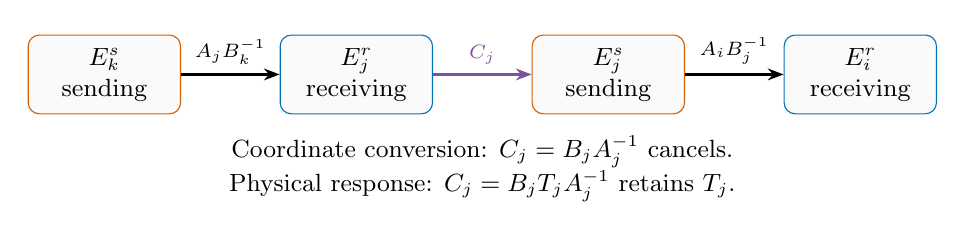
\begin{tikzpicture}
\node[box,draw=send,text width=17mm] (ks) at (0,0) {$E_k^s$\\sending};
\node[box,draw=receive,text width=17mm] (jr) at (3.2,0) {$E_j^r$\\receiving};
\node[box,draw=send,text width=17mm] (js) at (6.4,0) {$E_j^s$\\sending};
\node[box,draw=receive,text width=17mm] (ir) at (9.6,0) {$E_i^r$\\receiving};
\draw[arr] (ks) -- node[above,font=\scriptsize] {$A_jB_k^{-1}$} (jr);
\draw[arr,violet] (jr) -- node[above,font=\scriptsize] {$C_j$} (js);
\draw[arr] (js) -- node[above,font=\scriptsize] {$A_iB_j^{-1}$} (ir);
\node[align=center] at (4.8,-1.2)
{Coordinate conversion: $C_j=B_jA_j^{-1}$ cancels.\\
Physical response: $C_j=B_jT_jA_j^{-1}$ retains $T_j$.};
\end{tikzpicture}
\caption{\textbf{Role spaces require a handoff.} Canonical coordinate conversion eliminates the apparent extra transport. A noncanonical response introduces actual model structure.}
\end{figure}

\section{Partner-specific frames}
For each relationship $\{i,j\}$ introduce endpoint maps from an edge reference space:
\begin{equation}
 \Omega_{ij}=U_{i|j}U_{j|i}^{-1}.
 \label{eq:partner}
\end{equation}
Agent 1 can use a different endpoint frame with agent 3 than with agent 23. If the same endpoint factors serve both directions, $\Omega_{ji}=\Omega_{ij}^{-1}$, but triangle cancellation fails because a vertex's factors differ by partner. Independently directed role factors release even that reversal constraint.

A common right action on both endpoint factors,
\begin{equation}
 U_{i|j}\mapsto U_{i|j}h_{ij},\qquad U_{j|i}\mapsto U_{j|i}h_{ij},
\end{equation}
leaves the link unchanged. Without other endpoint-dependent terms, only their product matters. An independent link is then a more economical representation. A frame attached to a token type, occurrence, position pair, or inferred contextual edge gives a different model and storage cost.

The mean cross term factors pairwise as
\begin{equation}
 \mu_i^\top\Omega_{ij}^{-\top}\Sigma_j^{-1}\mu_j
 =(U_{i|j}^{-1}\mu_i)^\top(U_{j|i}^\top\Sigma_j^{-1}\mu_j).
\end{equation}
Both vectors depend on the pair. This is not generally one reusable $Q_i$ and $K_j$. More relational freedom does not automatically reduce computation.



\section{One frame with subspaces and functional operators}
\label{sec:subspaces}
A common frame need not make every interaction use every direction. Let $\bar{\mathsf P}_i$ be a reference projector and define
\begin{equation}
 \mathsf P_i=U_i\bar{\mathsf P}_iU_i^{-1}.
\end{equation}
Then $\mathsf P_i^2=\mathsf P_i$, $\im\mathsf P_i=U_i\im\bar{\mathsf P}_i$, and $\mathsf P_i'=g_i\mathsf P_ig_i^{-1}$. Different role projectors can overlap and need not sum to identity. Their interpretation comes from the objective and observed behavior, not from naming coordinate blocks as faculties.

\subsection{A metric is required for orthogonality}
Let $G_i\succ0$ be a metric, transforming as $G_i'=g_i^{-\top}G_ig_i^{-1}$. For a full-column-rank basis $Z_i\in\R^{d\times r}$,
\begin{equation}
 \boxed{\mathsf P_i=Z_i(Z_i^\top G_iZ_i)^{-1}Z_i^\top G_i.}
 \label{eq:metric-proj}
\end{equation}
The Gram matrix is SPD because $a^\top Z_i^\top G_iZ_ia>0$ for $a\ne0$. Multiplication proves $\mathsf P_i^2=\mathsf P_i$, $\mathsf P_iZ_i=Z_i$, and $\mathsf P_i^\top G_i=G_i\mathsf P_i$. Under $Z_i'=g_iZ_i$, the Gram matrix is unchanged and the projector transforms by conjugation.

For example,
\begin{equation}
 \mathsf P=\begin{pmatrix}1&0\\0&0\end{pmatrix},\quad
 g=\begin{pmatrix}1&1\\0&1\end{pmatrix}
 \quad\Longrightarrow\quad
 \mathsf P'=\begin{pmatrix}1&-1\\0&0\end{pmatrix},\quad
 G'=\begin{pmatrix}1&-1\\-1&2\end{pmatrix}.
\end{equation}
The new projector is not Euclidean symmetric, but remains $G'$-orthogonal. Requiring numerical Euclidean symmetry after arbitrary $\GL(d)$ changes mixes conventions.

If $G_i=U_i^{-\top}G_0U_i^{-1}$, then flat transport is metric-isometric:
\begin{equation}
 \Omega_{ij}^\top G_i\Omega_{ij}=G_j.
\end{equation}
Nonorthogonal numerical frames can thus represent isometric coordinate conversion. Stretch relative to a fixed physical metric is a separate active choice.

\begin{figure}[tb]
\centering
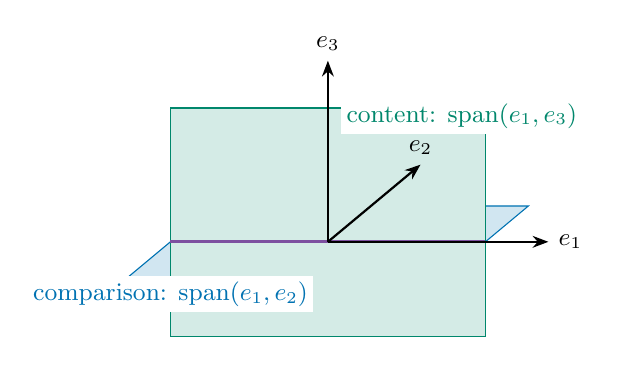
\begin{tikzpicture}[x={(1cm,0cm)},y={(0.42cm,0.35cm)},z={(0cm,1cm)}]
\filldraw[fill=receive!18,draw=receive] (-2,-1.3,0)--(2,-1.3,0)--(2,1.3,0)--(-2,1.3,0)--cycle;
\filldraw[fill=content!17,draw=content] (-2,0,-1.2)--(2,0,-1.2)--(2,0,1.7)--(-2,0,1.7)--cycle;
\draw[very thick,violet] (-2,0,0)--(2,0,0);
\draw[arr] (0,0,0)--(2.8,0,0) node[right] {$e_1$};
\draw[arr] (0,0,0)--(0,2.8,0) node[above] {$e_2$};
\draw[arr] (0,0,0)--(0,0,2.3) node[above] {$e_3$};
\node[receive,fill=white,inner sep=2pt] at (-1.2,-1.9,0) {comparison: $\operatorname{span}(e_1,e_2)$};
\node[content,fill=white,inner sep=2pt] at (1.7,0,1.6) {content: $\operatorname{span}(e_1,e_3)$};
\end{tikzpicture}
\caption{\textbf{Overlapping functions in one reference frame.} The two planes share the $e_1$ direction. They are illustrative learned or specified selections, without cognitive labels. Under a local frame $U_i$, both planes transform together into $E_i$; a metric specifies what their orthogonal projections mean.}
\label{fig:planes}
\end{figure}

\subsection{Rectangular measurements and nonsingular marginals}
A projector and a readout are distinct. Let $L_i:E_i\to\R^r$ have full row rank. The exact marginal is
\begin{equation}
 (L_i)_\#q_i=\mathcal N(L_i\mu_i,L_i\Sigma_iL_i^\top).
\end{equation}
It is nonsingular because $L_i^\top a\ne0$ for $a\ne0$. An ambient rank-deficient projector instead gives a singular $d$-dimensional covariance. Use coordinates on its image rather than inserting a zero determinant into \eqref{eq:gausskl}. Two singular measures with different affine supports can even have infinite KL.

The metric projector associated with $L_i$ is
\begin{equation}
 \mathsf P_i=G_i^{-1}L_i^\top(L_iG_i^{-1}L_i^\top)^{-1}L_i.
\end{equation}
It has kernel $\ker L_i$ and satisfies $L_i\mathsf P_i=L_i$. Reparameterizing the output by any invertible $h_i$ leaves this projector unchanged.

Compare both beliefs in the receiver's measured space:
\begin{equation}
 D^L_{ij}=\KL\left((L_i)_\#q_i\,
 \middle\|\,(L_i\Omega_{ij})_\#q_j\right).
 \label{eq:projected}
\end{equation}
The law $L_i'=h_iL_ig_i^{-1}$ gives a common invertible $h_i$ on both operands, preserving the score. For $r=d$ and invertible $L_i$, $D^L_{ij}=D_{ij}$ exactly. A common invertible measurement cannot change KL relevance. At $r<d$, completing $L_i$ to an invertible coordinate map and applying the KL chain rule gives
\begin{equation}
 D_{ij}-D^L_{ij}
 =\E_{Y\sim(L_i)_\#q_i}
 \KL\big(q_i(Z\mid Y)\,\|\,(\Omega_{ij\#}q_j)(Z\mid Y)\big)\ge0.
 \label{eq:lost-kl}
\end{equation}
The complementary coordinates are denoted $Z$ here. The lost term quantifies the comparison information discarded.

For a concrete two-dimensional example, let $\mu_i=(1,1)^\top$, source means $(1,1)^\top,(1,-1)^\top$, and all covariances be identity, with identity transport. Full KL costs are $(0,2)$; $L=(1,0)$ gives costs $(0,0)$. At unit temperature and equal priors, the weights change from $(0.8808,0.1192)$ to $(0.5,0.5)$. Content $T=(0,1)$ can still distinguish values $+1$ and $-1$, but the selected comparison no longer chooses between them. Information removal is a functional choice with possible costs.

\subsection{A general value is more than a projection}
A restricted channel can be
\begin{equation}
 \mathcal C_{ij}=\beta_{ij}\mathsf P_i^{r}\Omega_{ij}\mathsf P_j^{s},
 \qquad
 \rank\mathcal C_{ij}\le
 \min(\rank\mathsf P_i^r,\rank\mathsf P_j^s).
 \label{eq:restricted-channel}
\end{equation}
It is covariant if the projectors and transport obey their laws and $\beta_{ij}$ is invariant. Under metric-orthogonal projections and isometric transport its induced norm is at most $\beta_{ij}$. Such a channel cannot represent $2\beta_{ij}\Omega_{ij}$. Oblique projectors do not obey this contraction bound.

A general one-frame content map instead has the form
\begin{equation}
 \mathcal C_{ij}=\beta_{ij}U_iBU_j^{-1},\qquad B=OT,
 \label{eq:body-content}
\end{equation}
where $T:\R^d\to\R^s$ selects and mixes source content and $O:\R^s\to\R^d$ places it in the receiver. $B$ can attenuate, amplify, rotate, mix, or suppress directions. Its image and kernel are subspaces; the operator additionally specifies strengths and correspondences. With Euclidean orthonormal bases $Z_s,Z_r$, the factorization $B=Z_rDZ_s^\top$ separates source extraction, channel mixing $D$, and receiver placement.

\begin{figure}[tb]
\centering
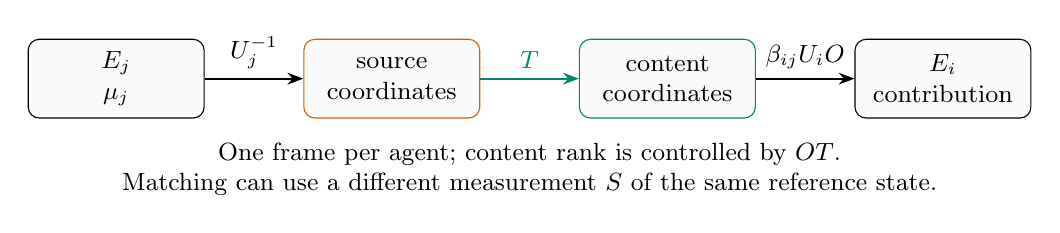
\begin{tikzpicture}
\node[box,text width=20mm] (a) at (0,0) {$E_j$\\$\mu_j$};
\node[box,text width=20mm,draw=send] (b) at (3.5,0) {source\\coordinates};
\node[box,text width=20mm,draw=content] (c) at (7,0) {content\\coordinates};
\node[box,text width=20mm] (d) at (10.5,0) {$E_i$\\contribution};
\draw[arr] (a)--node[above] {$U_j^{-1}$}(b);
\draw[arr,content] (b)--node[above] {$T$}(c);
\draw[arr] (c)--node[above] {$\beta_{ij}U_iO$}(d);
\node[align=center] at (5.25,-1.15) {One frame per agent; content rank is controlled by $OT$.\\
Matching can use a different measurement $S$ of the same reference state.};
\end{tikzpicture}
\caption{\textbf{Functional readouts do not require additional frames.} A rectangular extraction can lose information, and a channel can change strengths. Neither operation is generically an invertible gauge transformation.}
\end{figure}

Even one-dimensional selections show a directional effect. For $e_1$-projection $\mathsf P$ and a planar rotation $R_\theta$,
\begin{equation}
 \mathsf PR_\theta\mathsf P=
 \begin{pmatrix}\cos\theta&0\\0&0\end{pmatrix}.
\end{equation}
The surviving direction changes gain and vanishes at $\theta=\pi/2$, although $R_\theta$ remains invertible. More generally, if $Z_i,Z_j$ are orthonormal $r$-frames and $\Omega_{ij}$ is orthogonal, the compressed map is $Z_i^\top\Omega_{ij}Z_j$. Its singular values are cosines of principal angles between the selected subspaces \cite{Edelman1998}. Singular-value attenuation and orientation are distinct from the scalar attention weight.

\subsection{Fixed invariant subspaces versus transforming subspaces}
Passive covariance permits an arbitrary transforming projector field. A fixed numerical projector invariant under every active group action must satisfy
\begin{equation}
 \mathsf P\rho(g)=\rho(g)\mathsf P\quad\text{for all }g.
\end{equation}
For the defining $\GL(d)$ representation, commuting with diagonal matrices makes $\mathsf P$ diagonal and commuting with shears makes every diagonal entry equal. Idempotence leaves only $0$ and $I$. The defining real $\SO(d)$ representation for $d\ge2$ likewise has no nontrivial invariant image: rotations of any nonzero vector span the whole space.

This statement about projectors is not a scalar-only version of real Schur's lemma. The $\SO(2)$ commutant includes $aI+bJ$, with $J$ the $90^\circ$ rotation; its idempotents are still only $0,I$. General real irreducible commutants can have real, complex, or quaternionic type. Complete reducibility must be stated, rather than assumed for arbitrary representations.

Multiplicity spaces can support invariant selection. For $\rho(g)=I_m\otimes g$, where the defining commutant is scalar,
\begin{equation}
 \operatorname{End}_{G}(\R^m\otimes\R^d)
 =\{B\otimes I_d:B\in\R^{m\times m}\}.
\end{equation}
Projectors can select combinations of copies while retaining entire representation factors. Independently transforming copies generally remove this mixing freedom. These restrictions connect to equivariant linear-layer design \cite{Finzi2021}; they do not show that learned transformer heads must be irreducible physical sectors.

An unlabeled state-dependent proposal uses $T_i=\Sigma_iG_i$, which transforms by conjugation and is $G_i$-self-adjoint. It is similar to the SPD matrix $G_i^{1/2}\Sigma_iG_i^{1/2}$. A spectral projector onto a separated eigenvalue cluster is covariant. For distinct eigenvalues,
\begin{equation}
 \mathsf P_a=\prod_{\lambda_b\ne\lambda_a}
 \frac{T_i-\lambda_bI}{\lambda_a-\lambda_b}.
\end{equation}
Summing selected eigenspaces gives a cluster projector. Selecting the largest $r$ eigenvalues is unambiguous at a gap $\lambda_r>\lambda_{r+1}$. Choosing these uncertainty directions for communication is a hypothesis, not a consequence of covariance. At $T_i=cI$, a nontrivial fixed-rank selection cannot follow equivariantly from this tensor alone because its rotational stabilizer forbids it. Extra structure or explicit symmetry breaking is necessary.

Finally, reference relabeling matters: under $U_i\mapsto U_ih$, preserve physical operators by $\bar{\mathsf P}_i\mapsto h^{-1}\bar{\mathsf P}_ih$ and $B\mapsto h^{-1}Bh$. Holding reference operators fixed restricts that redundancy to their common stabilizer.

\section{When projected comparison defines quotient transport}
\label{sec:quotient}
The score \eqref{eq:projected} is valid without any transport between reduced source and receiver spaces. The stronger construction needs a compatibility condition.

\begin{proposition}[Descent criterion]
For surjective $L_j:E_j\to S_j$ and $L_i:E_i\to S_i$, a unique map $\bar\Omega_{ij}:S_j\to S_i$ satisfying
\begin{equation}
 L_i\Omega_{ij}=\bar\Omega_{ij}L_j
 \label{eq:descent}
\end{equation}
exists if and only if $\Omega_{ij}\ker L_j\subseteq\ker L_i$.
\end{proposition}
\begin{proof}
Apply \eqref{eq:descent} to an element of $\ker L_j$ for necessity. Conversely define $\bar\Omega_{ij}(L_jx)=L_i\Omega_{ij}x$. Kernel inclusion makes this independent of representative; surjectivity gives uniqueness.
\end{proof}
With equal ambient and quotient dimensions at both endpoints and invertible $\Omega_{ij}$, inclusion becomes equality by dimension, and the induced map is invertible.

For $L_i=L_j=(1,0)$ and $\Omega_{ij}=R_{\pi/2}$, the discarded vector $e_2$ maps to $-e_1$. Thus the same reduced source coordinate can produce different reduced receiver coordinates; no quotient transport exists. Projected Gaussian comparison is still well-defined.

\begin{figure}[tb]
\centering
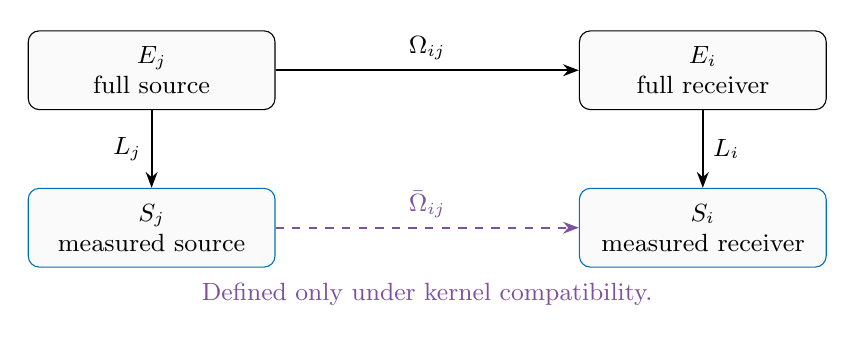
\begin{tikzpicture}
\node[box] (ej) at (0,2) {$E_j$\\full source};
\node[box] (ei) at (7,2) {$E_i$\\full receiver};
\node[box,draw=receive] (sj) at (0,0) {$S_j$\\measured source};
\node[box,draw=receive] (si) at (7,0) {$S_i$\\measured receiver};
\draw[arr] (ej)--node[above] {$\Omega_{ij}$}(ei);
\draw[arr] (ej)--node[left] {$L_j$}(sj);
\draw[arr] (ei)--node[right] {$L_i$}(si);
\draw[arr,dashed,violet] (sj)--node[above] {$\bar\Omega_{ij}$}(si);
\node[violet] at (3.5,-0.85) {Defined only under kernel compatibility.};
\end{tikzpicture}
\caption{\textbf{A measurement is not automatically a quotient connection.} The dashed map exists precisely when discarded source directions remain discarded after transport. Receiver-projected comparison uses the top and right arrows and needs no dashed map.}
\end{figure}

If quotient maps exist on every edge, their compositions follow ambient compositions by surjectivity. A flat ambient connection then induces a flat quotient connection. A parallel projector transported from a basepoint is path-independent precisely when it commutes with every based holonomy. For its image alone, holonomy invariance of that subspace suffices; a commuting projector also needs an invariant complement. Metric-preserving holonomy preserves the orthogonal complement automatically. These are the global obligations for a transport-compatible subspace field.

\section{Mixture prediction, precision pooling, and finite updates}
\label{sec:aggregation}
The expression $\sum_j\beta_{ij}v_j$ occurs in different models. Their covariances and dynamical meanings distinguish them.

For a source mixture, $J\sim\beta_i$ and $Z\mid J=j\sim\mathcal N(m_{ij},C_{ij})$, the predictive moments are
\begin{align}
 \bar m_i&=\sum_j\beta_{ij}m_{ij},\\
 \Cov(Z)&=\sum_j\beta_{ij}
 [C_{ij}+(m_{ij}-\bar m_i)(m_{ij}-\bar m_i)^\top].
 \label{eq:mixture}
\end{align}
For independent draws $Z_j$ and $Z=\sum_j\beta_{ij}Z_j$, the mean is the same but covariance is $\sum_j\beta_{ij}^2C_{ij}$. Correlated draws add the appropriate cross-covariance terms. These are different random variables.

By contrast, minimize $\sum_j\beta_{ij}\KL(q\|p_{ij})$ with sources and weights fixed. The normalized geometric product $p_*\propto\prod_jp_{ij}^{\beta_{ij}}$ gives an exact KL gap, hence the unique optimum. For Gaussian sources,
\begin{equation}
 \boxed{\Sigma_*^{-1}=\sum_j\beta_{ij}C_{ij}^{-1},\qquad
 \mu_*=\left(\sum_j\beta_{ij}C_{ij}^{-1}\right)^{-1}
 \sum_j\beta_{ij}C_{ij}^{-1}m_{ij}.}
 \label{eq:precision}
\end{equation}
The mean equals the arithmetic mixture mean when all source precisions agree, but not generally. With a prior KL coefficient $\alpha>0$ and pair coefficient $\lambda>0$, the optimum precision is
\begin{equation}
 \Sigma_*^{-1}=
 \frac{\alpha H_0+\lambda\sum_j\beta_{ij}H_{ij}}{\alpha+\lambda},
\end{equation}
while its mean solves the information-vector system using numerator precision. The denominator records the entropy coefficient in this weighted sum of KLs. A different product-likelihood objective can have a different coefficient.

A finite filtering step is another operation. With frozen templates and routing for the indicated partial derivative,
\begin{equation}
 g_i=\alpha H_0(\mu_i-\mu_0)
 +\lambda\sum_j\beta_{ij}H_{ij}(\mu_i-m_{ij}),\qquad
 \mu_i^+=\mu_i-\eta\Sigma_i g_i.
 \label{eq:ng}
\end{equation}
The Gaussian mean Fisher metric is $\Sigma_i^{-1}$, so $\Sigma_i g_i$ is the natural gradient. If $\alpha=0$, every $C_{ij}=\Sigma_i$, and $\eta\lambda=1$, this single step reaches the mixture mean. In general it does not. Trust bounds and clipping alter it further. Differentiating through routing after deleting its entropy term, or differentiating other receivers' rows, requires additional terms.

For scalar sources $\mathcal N(0,1)$ and $\mathcal N(2,4)$ with equal weights, the mixture has mean $1$ and variance $3.5$. The precision pool has mean $0.4$ and variance $1.6$. A weighted independent draw has mean $1$ and variance $1.25$.

\begin{figure}[tb]
\centering
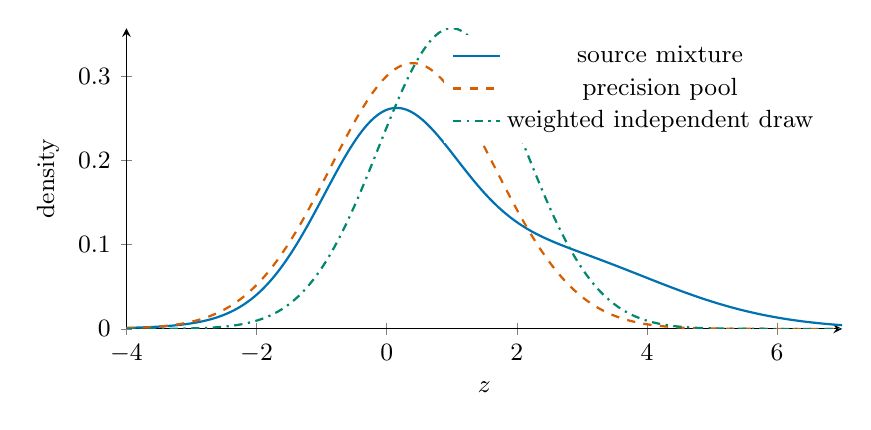
\begin{tikzpicture}
\begin{axis}[width=0.88\textwidth,height=5.4cm,xmin=-4,xmax=7,ymin=0,
 xlabel={$z$},ylabel={density},samples=180,domain=-4:7,
 legend style={font=\small,at={(0.98,0.98)},anchor=north east,draw=none,fill=white},
 axis lines=left]
\addplot[receive,thick]{0.5*exp(-x^2/2)/sqrt(2*pi)+0.5*exp(-(x-2)^2/8)/sqrt(8*pi)};
\addlegendentry{source mixture}
\addplot[send,thick,dashed]{exp(-(x-0.4)^2/3.2)/sqrt(3.2*pi)};
\addlegendentry{precision pool}
\addplot[content,thick,dashdotted]{exp(-(x-1)^2/2.5)/sqrt(2.5*pi)};
\addlegendentry{weighted independent draw}
\end{axis}
\end{tikzpicture}
\caption{\textbf{Identical source weights do not specify an aggregation law.} The mixture selects a source, the precision pool minimizes a weighted $\KL(q\|p_j)$ objective, and the independent-draw law averages samples. The plotted densities use the exact scalar example in the text.}
\label{fig:pool}
\end{figure}

\section{Independent values without a third frame}
\label{sec:source-content}
The existing correspondence C3 provides a normalized probabilistic model for arbitrary attention values. Gaussian-key models also occur in the wider attention literature \cite{Nguyen2022}; the point here is the exact local construction and its limits.

\subsection{Separate conditional comparison and content}
Fix reference query $q_i\in\R^r$, keys $k_j\in\R^r$, values $v_j\in\R^s$, biases $b_{ij}$, $\tau>0$, and $R\in\SPD(s)$. All depend only on the declared conditioning context. Define
\begin{equation}
 D_i^{\rm prior}=\sum_j e^{b_{ij}+\|k_j\|^2/(2\tau)},\qquad
 \pi_{ij}=\frac{e^{b_{ij}+\|k_j\|^2/(2\tau)}}{D_i^{\rm prior}},
\end{equation}
and the joint density
\begin{equation}
 p_i(j,y,z)=\pi_{ij}\varphi_{\tau I_r}(y-k_j)\varphi_R(z-v_j).
 \label{eq:joint}
\end{equation}
Counting measure and coordinate Lebesgue measures are understood. Each factor normalizes, so the joint does. Bayes' rule at the auxiliary comparison observation $Y=q_i$ gives
\begin{equation}
 a_{ij}=p(J=j\mid Y=q_i)=
 \softmax_j(q_i^\top k_j/\tau+b_{ij}),\qquad
 \E[Z\mid Y=q_i]=\sum_j a_{ij}v_j.
 \label{eq:predictive}
\end{equation}
The key-norm prior compensates the Gaussian source-energy term. A uniform prior would instead retain the key penalty of \eqref{eq:so}.

For the structured family $r(j,z)=\rho_j\varphi_R(z-v_j)$, direct cancellation gives
\begin{equation}
 \E_r[\log r-\log p_i(J,q_i,Z)]
 =\KL(\rho\|a_i)-\log p_i(q_i).
 \label{eq:structured}
\end{equation}
This is an exact posterior family, not an independent mean-field approximation. Taking $q_i=W_Qx_i$, $k_j=W_Kx_j$, $v_j=W_Vx_j$ and applying $W_O$ recovers a finite vanilla head, including rectangular or singular maps. The content covariance is declared in its own space, so a singular $W_V$ causes no density singularity.

The evidence retains all normalizers:
\begin{equation}
 -\log p_i(q_i)=\frac r2\log(2\pi\tau)+\frac{\|q_i\|^2}{2\tau}
 +\log D_i^{\rm prior}
 -\log\sum_j e^{q_i^\top k_j/\tau+b_{ij}}.
\end{equation}
At fixed context this contains no $v_j$ or $W_O$. It cannot learn useful values by itself. A content observation or predictive objective must identify them. Conditioning on a downstream target generally changes exact source inference; ordinary forward attention need not equal that target-conditioned posterior.

Replacing the structured family by $\rho_jq(z)$ incurs an additional term
$\sum_j\rho_j\KL(q(z)\|\mathcal N(v_j,R))$. Its Gaussian optimum at fixed $\rho$ has mean $\bar v_\rho$ and covariance $R$, but leaves
\begin{equation}
 \frac12\sum_j\rho_j(v_j-\bar v_\rho)^\top R^{-1}(v_j-\bar v_\rho).
\end{equation}
Thus values can affect routing under that altered approximation. Variational-family structure matters \cite{Blei2017}.

\subsection{Measurements of the same random belief}
One frame gives reference belief $\mathcal N(\xi_j,C_j)$. A comparison map $S$ and content map $T$ can act on this state without any third frame. But two possible joint laws must be distinguished.

If $Z\mid J=j\sim\mathcal N(\xi_j,C_j)$ is a shared latent draw and
\begin{equation}
 Y=SZ+\varepsilon,\quad \varepsilon\sim\mathcal N(0,R_y),\quad
 V=TZ,
\end{equation}
with independent noise, $R_y\succeq0$, and $R_j^Y=SC_jS^\top+R_y\succ0$, Gaussian conditioning gives
\begin{equation}
 \boxed{\E[V\mid Y=y,J=j]=
 T\xi_j+TC_jS^\top(R_j^Y)^{-1}(y-S\xi_j).}
 \label{eq:conditional-value}
\end{equation}
Its covariance is
\begin{equation}
 TC_jT^\top-TC_jS^\top(R_j^Y)^{-1}SC_jT^\top.
 \label{eq:conditional-cov}
\end{equation}
This matrix can be singular, which is permitted for the conditional moment statement. The exact posterior over $J$ is proportional to
$\pi_j\varphi_{R_j^Y}(y-S\xi_j)$, and the total predictive content averages \eqref{eq:conditional-value} using those weights.

The derivation follows from the joint Gaussian block covariance
\begin{equation}
 \Cov\begin{pmatrix}Y\\V\end{pmatrix}\Bigm|J=j
 =\begin{pmatrix}
 R_j^Y&SC_jT^\top\\
 TC_jS^\top&TC_jT^\top
 \end{pmatrix},
\end{equation}
followed by completing the conditional square, or by subtracting the linear regression residual. Since $R_j^Y$ is invertible, the content is $T\xi_j$ for every $y$ if and only if $TC_jS^\top=0$. This is conditional covariance orthogonality, equivalent to $V\perp Y\mid J=j$ for this Gaussian model. Mixing over $J$ can still create dependence.

Euclidean orthogonality of rows is insufficient. With $S=(1,0)$, $T=(0,1)$ and
\begin{equation}
 C_j=\begin{pmatrix}1&\rho\\\rho&1\end{pmatrix},\qquad |\rho|<1,
\end{equation}
zero observation noise gives conditional content mean
$\xi_{j,2}+\rho(y-\xi_{j,1})$. Orthogonal coordinate axes remain statistically correlated when $\rho\ne0$.

\begin{figure}[tb]
\centering
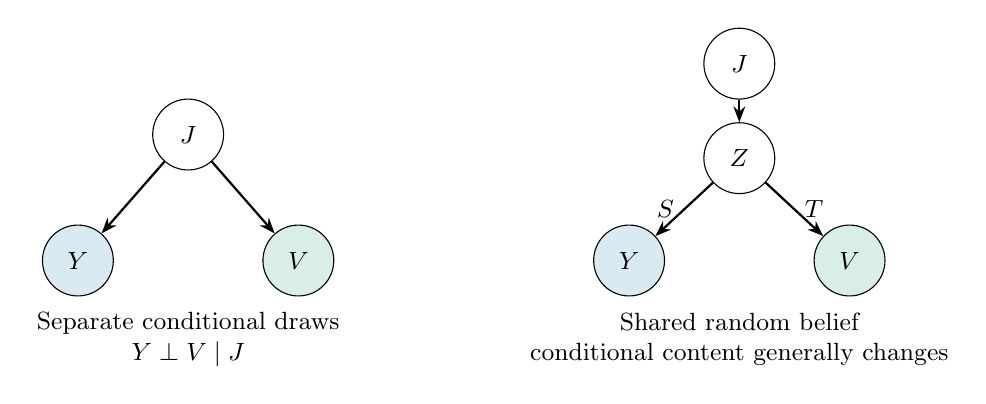
\begin{tikzpicture}
\tikzset{rv/.style={circle,draw,minimum size=9mm}}
\node[rv] (j1) at (0,1.6) {$J$};
\node[rv,fill=receive!15] (y1) at (-1.4,0) {$Y$};
\node[rv,fill=content!15] (v1) at (1.4,0) {$V$};
\draw[arr] (j1)--(y1);
\draw[arr] (j1)--(v1);
\node[align=center] at (0,-1) {Separate conditional draws\\$Y\perp V\mid J$};
\node[rv] (j2) at (7,2.5) {$J$};
\node[rv] (z2) at (7,1.3) {$Z$};
\node[rv,fill=receive!15] (y2) at (5.6,0) {$Y$};
\node[rv,fill=content!15] (v2) at (8.4,0) {$V$};
\draw[arr] (j2)--(z2);
\draw[arr] (z2)--node[left] {$S$}(y2);
\draw[arr] (z2)--node[right] {$T$}(v2);
\node[align=center] at (7,-1) {Shared random belief\\conditional content generally changes};
\end{tikzpicture}
\caption{\textbf{Two different meanings of one underlying state.} On the left, source-conditioned content is independent of the comparison observation. On the right, the two readouts share a latent draw and acquire the conditional correction in \eqref{eq:conditional-value}. Both can use one reference frame; their probability laws differ.}
\end{figure}

\subsection{Uncertain comparison instead of a point observation}
A projected-KL router also has a normalized conditional-content construction. Let $\widehat q_i$ be the fixed receiver comparison distribution, $p_j^S$ normalized comparison densities, and $r_j$ normalized content laws. Set
\begin{equation}
 p(j,y,z)=\pi_jp_j^S(y)r_j(z),\qquad
 r_\beta(j,y,z)=\beta_j\widehat q_i(y)r_j(z).
\end{equation}
Successive integration proves normalization, and direct expectation gives
\begin{equation}
 \KL(r_\beta\|p)=
 \sum_j\beta_j\KL(\widehat q_i\|p_j^S)+\KL(\beta\|\pi).
\end{equation}
At temperature one, optimizing $\beta$ recovers projected-KL attention. Its variational content mean is $\sum_j\beta_j\E_{r_j}Z$. This is a restricted variational optimum, whereas \eqref{eq:predictive} is an exact posterior given a point observation. The supplied receiver distribution and its objective remain modeling inputs.

\subsection{Why independent values do not guarantee one free-energy flow}
The existing C5 obstruction is short. Let a variable query $q\in\R^2$ attend to keys $\pm(1,0)^\top$ and values $\pm(0,1)^\top$ at unit temperature and zero bias. The attention increment is
\begin{equation}
 f(q)=(0,\tanh q_1)^\top,\qquad Df(0)=
 N=\begin{pmatrix}0&0\\1&0\end{pmatrix}.
\end{equation}
Suppose $f=-G^{-1}\nabla E$ near zero for smooth SPD $G$ and $C^2$ energy $E$. Since $f(0)=0$, $\nabla^2E(0)=-G(0)N$. For $G(0)=\left(\begin{smallmatrix}a&b\\b&c\end{smallmatrix}\right)$, Hessian symmetry forces $c=0$, contradicting SPD. Thus every arbitrary independent-value attention increment cannot be a natural-gradient flow on the same query state.

A separate content state is different. At fixed weights, the objective
\begin{equation}
 E(m)=\frac12\sum_j a_j(m-v_j)^\top R^{-1}(m-v_j)
\end{equation}
has Gaussian-mean natural gradient $m-\bar v$. A unit step reaches $\bar v$. This conditional construction neither identifies $m$ with the query nor differentiates through changing routing. The normalized prediction model and the same-state gradient obstruction are compatible. Specifying which state is updated is necessary before attaching a meaning such as internalization.



\section{A concrete family to investigate}
\label{sec:family}
The discussion can be expressed as a finite family with one frame per agent. Let $\xi_i=U_i^{-1}\mu_i$, $C_i=U_i^{-1}\Sigma_iU_i^{-\top}$, choose a full-row-rank comparison map $S:\R^d\to\R^r$, and choose content maps $T:\R^d\to\R^s$, $O:\R^s\to\R^d$. Define
\begin{align}
 D^S_{ij}&=\KL\big(\mathcal N(S\xi_i,SC_iS^\top)
 \,\|\,\mathcal N(S\xi_j,SC_jS^\top)\big),\\
 \beta_{ij}&=\softmax_j(-D^S_{ij}/\tau+\log\pi_{ij}),\\
 m_i^{\rm content}&=U_iO\sum_j\beta_{ij}T\xi_j.
 \label{eq:family}
\end{align}
All densities are well-defined, and local passive covariance follows because the reference coordinates are unchanged. The score is an exact marginal KL and the output is an exact declared mixture moment. Section \ref{sec:source-content} gives a normalized independent-content realization at temperature one and identifies the stronger corrections for shared latent draws. Equation \eqref{eq:family} alone does not specify learning or receiver-state dynamics.

This family has transparent limits. $S=I$ restores full Gaussian matching. $OT=I$ restores full transported content. Both recover the original score-plus-mixture-readout pair, without claiming that this pair equals the implemented filtering step. Rank reduction in $S$ changes what is compared; rank reduction in $OT$ changes what can be transmitted. Equal isotropic comparison covariances give squared-distance attention, and equal key norms additionally give dot-product weights.

Two role maps $S_Q,S_K$ can be introduced in the same reference frame to compare distinct Gaussian measurements:
\begin{equation}
 \KL\big(\mathcal N(S_Q\xi_i,S_QC_iS_Q^\top)
 \,\|\,\mathcal N(S_K\xi_j,S_KC_jS_K^\top)\big).
 \label{eq:role-measure}
\end{equation}
Both measurements must land in the same comparison space and have full row rank for nonsingular densities. Unlike an invertible common $S$, separate maps can change even a full-dimensional score. They are added model parameters, and comparing distinct observables requires a modeling justification. Their mathematical validity does not show that the observed Q/K/V gains arise from such full-distribution measurements: the legacy QKV path maps means only, while the distinct relational path now evaluates full projected Gaussian marginals.

Pair-dependent content $B_{ij}$ or comparison maps could extend \eqref{eq:family}; independent links could additionally alter relational geometry. These are separate axes of capacity. An extension should first state which failure of the smaller family it addresses. Pairwise parameter count alone can overwhelm the intended economy of replacing shared linear maps.

\subsection{Whole-belief inputs with independent gauge blocks}
\label{sec:full-input-heads}
The partition used to represent gauge transformations need not restrict the coordinates available to an attention head. Let the belief dimension be $K=Hd$, and let $E_h:\R^d\to\R^K$ insert a vector into block $h$, with $E_h^\top E_g=\delta_{hg}I_d$ and $\sum_h E_hE_h^\top=I_K$. Independent block frames give
\begin{equation}
 U_i=\diag(U_i^{(1)},\ldots,U_i^{(H)}),\qquad
 \xi_i=U_i^{-1}\mu_i,\qquad C_i=U_i^{-1}\Sigma_iU_i^{-\top}.
\end{equation}
Each $U_i^{(h)}\in\GL(d)$ may depend on its own learned frame parameters. The token belief still has a $K$-dimensional mean. The block partition specifies how coordinates transform; restricting a readout to $E_h^\top\xi_i$ is an additional architectural choice.

For each attention head choose full-row-rank maps $S_Q^h,S_K^h:\R^K\to\R^r$, a content map $T_h:\R^K\to\R^s$, and an output map $O_h:\R^s\to\R^d$. The projected distributions and the declared mixture mean are
\begin{align}
 a_{Qi}^h&=S_Q^h\xi_i,& G_{Qi}^h&=S_Q^hC_i(S_Q^h)^\top,\\
 a_{Kj}^h&=S_K^h\xi_j,& G_{Kj}^h&=S_K^hC_j(S_K^h)^\top,\\
 D_{ij}^h&=\KL\big(\mathcal N(a_{Qi}^h,G_{Qi}^h)\|\mathcal N(a_{Kj}^h,G_{Kj}^h)\big),\\
 \beta_{ij}^h&=\softmax_{j\in\mathcal J_i}(-D_{ij}^h/\tau_h+\log\pi_{ij}^h),\\
 m_i^{\rm content}&=U_i\sum_{h=1}^H E_hO_h\sum_{j\in\mathcal J_i}\beta_{ij}^hT_h\xi_j.
 \label{eq:full-input-heads}
\end{align}
Here $\Sigma_i\succ0$, $\tau_h>0$, and the prior gives nonzero total mass to the finite support $\mathcal J_i$. Full row rank makes every projected covariance positive definite. The same comparison coordinates are used for the two roles of a head. Setting $S_A^h=\bar S_A^hE_h^\top$ and $T_h=\bar T_hE_h^\top$ recovers the restricted input family exactly. Dense rectangular maps permit overlapping readouts of all blocks without identifying their frame parameters.

Under a passive block gauge change $g_i=\diag(g_i^{(1)},\ldots,g_i^{(H)})$, take $U_i'=g_iU_i$, $\mu_i'=g_i\mu_i$, and $\Sigma_i'=g_i\Sigma_ig_i^\top$. Direct substitution gives $\xi_i'=\xi_i$ and $C_i'=C_i$. Thus the projected distributions, scores, and weights in \eqref{eq:full-input-heads} are unchanged, while $(m_i^{\rm content})'=g_i m_i^{\rm content}$. This calculation holds in the fixed reference coordinates used to define the learned maps. The maps need not commute with the physical block action, because they act after canonicalization. It is a covariance statement for the full-Gaussian construction; a locally diagonal covariance family is not closed under arbitrary $\GL(d)$ congruences, so this calculation does not certify equivariance of the approximate training dynamics.

Overlapping measurements of one random belief are generally correlated. For $X_i\sim\mathcal N(\xi_i,C_i)$,
\begin{equation}
 \Cov(S_Q^hX_i,S_Q^\ell X_i)=S_Q^h C_i(S_Q^\ell)^\top.
\end{equation}
The separate marginal KLs are well-defined even when this cross covariance is nonzero. Their sum is not thereby the joint KL of the stacked measurements, nor does it define a factorized ELBO. A joint interpretation must specify the correlations and a normalized model; the source/content qualifications of Section \ref{sec:source-content} continue to apply.

This construction gives each attention head access to the entire token representation, as in the input projections of standard multi-head attention \cite{Vaswani2017}. It does not equate the complete architectures. Equation \eqref{eq:full-input-heads} places each head output into its own $d$-coordinate block through $E_hO_h$, whereas a general transformer output projection can mix the concatenated head outputs. Gaussian KL routing and the implemented conditional natural-gradient update also differ from dot-product routing and direct value replacement.

\subsection{Implemented input scope and conditional update}
The relational implementation supports \texttt{relational\_input\_scope=full} and the historical \texttt{head} setting. The full setting uses independent comparison arrays of shape $(H,r,K)$ and learned content factors of shapes $(H,s,K)$ and $(H,d,s)$. Compact inverse frame blocks contract with the input columns of these arrays, so dense $K\times K$ frame storage is unnecessary. For $K=64$, $H=2$, and $r=s=32$, every comparison and content readout has 64 input coordinates and 32 output coordinates. The implementation retains equal gauge-block and attention-head counts, and bounds $r,s$ by $d$; these restrictions are implementation choices rather than requirements of the rectangular Gaussian construction.

Independent Q/K maps are free parameters initialized with orthonormal rows across the selected input width. Learned full-input content begins with zero off-block columns: at $s=d$ it reproduces identity content, and at $s<d$ it begins as a local rank-$s$ projector. The off-block columns remain trainable. Setting the content rank to \texttt{None} instead selects parameter-free identity content; expanding the comparison input alone does not introduce a learned value map. The shared-Q/K compatibility mode retains an orthonormal-row parameterization, and historical serialized configurations through schema 15 migrate to head-local input. Schema 16 introduced the scope field. Schema 17 gives full input a meaning when relational projections are off; older off-mode checkpoints retain historical head-local behavior. Schema 18 adds the role-frame selector and replays earlier checkpoints with tied frames.

The router retains the full $r\times r$ covariance of each projected marginal of the declared local Gaussian. If finite-precision Gram construction loses positive definiteness, the existing fallback reconstructs the failed entries from the source covariance and compact inverse frames in float64, using a QR factorization of the projected square root. It adds no jitter or covariance floor, and still rejects numerical row-rank loss. This numerical recovery does not impose an invertibility constraint on the learned comparison map.

The content factors change the transported mean template. They do not push the covariance through $O_hT_h$: the conditional update retains the existing transported diagonal variance. The inner derivative conditions on the pre-update routing and templates, then applies the configured natural gradient and trust bound to the receiver belief. Outer gradients through the operators and frames remain available. Accordingly, \eqref{eq:full-input-heads} specifies the associated mixture readout, not an assertion that one implemented E-step replaces the belief by that mean or optimizes a common unrestricted ELBO.

With independent Q/K and learned content, the full-input operators store $2HrK+Hs(K+d)$ scalars, compared with $2Hrd+2Hds$ for head-local input. At $K=64$, $H=2$, and $r=s=32$, these totals are 14,336 and 8,192. The unchanged output widths do not make this a parameter-matched comparison. Full-input projections also perform more arithmetic; no production throughput or perplexity improvement is established by the implementation tests.

Restricted input access is a plausible contributor to an optimization or predictive limitation, but the reported test-perplexity plateau near 50 is not evidence of a ceiling caused by that restriction. A discriminating experiment compares the two scopes at fixed data, code revision, seeds, output ranks, temperature convention, and training budget, reporting seed variability and the additional parameter and compute costs. Such an experiment remains to be run. Tiny-model checks establish that the new routing uses all input blocks, agrees with direct Gaussian calculations, and propagates cross-block gradients; they do not establish the proposed performance mechanism.


\subsection{Coupled independent query and key frames}
\label{sec:implemented-role-frames}
The selector \texttt{qk\_frame\_mode=independent} implements the two-role construction of Sections \ref{sec:twoframes} and \ref{sec:bridges}. Write $A_i=U_{Qi}$ and $B_i=U_{Ki}$. Each is a block-diagonal realized frame with its own token-type Lie-algebra parameters and the existing positional factors composed in the same order. The query table remains the belief frame; the key table begins as an exact clone and is then learned independently. The directed channel
\begin{equation}
 \Omega_{ij}=A_iB_j^{-1}
\end{equation}
supplies both comparison transport and transmitted content. This is a coupled role separation: the source mean and source covariance use the key frame throughout the conditional attention calculation. Operations on the receiver belief, including the optional coordinate MLP, retain the query frame.

For relational scoring, the two canonical moments are
\begin{align}
 \xi_i^Q&=A_i^{-1}\mu_i, & C_i^Q&=A_i^{-1}\Sigma_iA_i^{-\top},\\
 \xi_j^K&=B_j^{-1}\mu_j, & C_j^K&=B_j^{-1}\Sigma_jB_j^{-\top}.
\end{align}
Head $h$ compares the Gaussian marginals with means $S_Q^h\xi_i^Q$ and $S_K^h\xi_j^K$ and covariances $S_Q^hC_i^Q(S_Q^h)^\top$ and $S_K^hC_j^K(S_K^h)^\top$. Its source content uses $T_h\xi_j^K$ and enters the receiver through $A_iE_hO_h$. The mixture-readout expression in \eqref{eq:full-input-heads} therefore becomes
\begin{equation}
 m_i^{\rm content}=A_i\sum_h E_hO_h\sum_j\beta_{ij}^hT_h\xi_j^K.
\end{equation}
The same qualifications concerning conditional updates, transported diagonal variance, and correlations between overlapping marginals remain. Under a passive block gauge change, $A_i'=g_iA_i$ and $B_i'=g_iB_i$ imply $\Omega_{ij}'=g_i\Omega_{ij}g_j^{-1}$, and both role-canonical moments are unchanged when the full Gaussian moments transform by congruence. This algebra does not close the locally diagonal family under general congruences.

The implementation keeps each frame and its genuine inverse separately. The attention channel is marked as a two-role transport rather than a same-frame flat cocycle: $\Omega_{ii}=A_iB_i^{-1}$ need not be the identity, and ordinary composition need not give $\Omega_{ij}\Omega_{jk}=\Omega_{ik}$. The role-bridge identities of Section \ref{sec:bridges} still apply; this is not an independently parameterized connection on every edge. With tied roles, cloned-frame outputs recover the existing route, and the sum of the two role gradients recovers the tied-table gradient in the tested smooth regime. Subsequent optimization need not preserve that equality.

The key table uses the same configured geometric optimizer policy as the query table. Its separate learning rate, \texttt{m\_phi\_key\_lr}, inherits the query rate when omitted; zero freezes the key initialization. With vocabulary size $P$ and $H$ equal blocks, this adds $PK^2/H$ parameters. At $P=50257,K=64,H=2$, the added table contains $102{,}926{,}336$ scalars. Sharing initial values does not eliminate this capacity or its optimizer memory. Separate frames are admitted for the existing one-layer, one-E-step conditional routes: relational projection, mean-only QKV, and unprojected full input. Historical unprojected head-local filtering retains its own semantics and rejects independent frames.

\subsection{Full-input routing without learned role projections}
\label{sec:unprojected-full}
Full input also operates with \texttt{relational\_mode=off} and all three learned QKV flags disabled. The adapter then contributes no learned parameters. The score compares the complete $K$-coordinate diagonal Gaussian belief against the transported source, using the diagonal of the covariance congruence. With block transport, that scalar score is supplied to each runtime head, while head-specific priors, temperatures, and value-coordinate updates remain. The full-input temperature is $\kappa\sqrt K$, compared with $\kappa\sqrt d$ for historical head-local comparison. This is the named unprojected full-input conditional-filtering route; it does not silently preserve the historical shared-objective update when the scope changes.

There are two distinct ways to expose cross-block information. Full-input scoring reads all blocks while leaving value transport block diagonal. Alternatively, complete \texttt{cross\_couplings} enlarges the frame algebra to $\mathfrak{gl}(K)$, allowing cross-block value transport and collapsing the implementation to one runtime attention head. The latter requires compatible headless priors and disables the HeadMixer and prior-bank evidence mixer. It also changes frame capacity and the interpretation of the head count. Because the admitted conditional route retains diagonal covariance, this dense-transport option remains an approximation to full Gaussian congruence; exact geometry should not be inferred from merely enabling the switch.

\subsection{Relationship to the legacy QKV implementation}
At the inspected repository revision, the QKV implementation already has the common-frame operator form
\begin{equation}
 T_i^A=I+U_i\Delta_AU_i^{-1}
 =U_i(I+\Delta_A)U_i^{-1},\qquad A\in\{Q,K,V\}.
 \label{eq:live-map}
\end{equation}
The square residual $\Delta_A$ is shared within a head across token positions and types. It need not be invertible or idempotent. Consequently it is a general endomorphism, not another gauge frame or necessarily a subspace projector. This existing path already tests functional role maps inside one realized frame.

The path maps means while leaving their local variances unchanged. With diagonal variances $s_i$, its router uses mapped receiver mean $a_i=T_i^Q\mu_i$, source mean $k_{ij}=\Omega_{ij}T_j^K\mu_j$, and
\begin{equation}
 d_{ij,k}=\sum_\ell\Omega_{ij,k\ell}^2s_{j,\ell}.
\end{equation}
Away from floors and clipping, the energy is
\begin{equation}
 E_{ij}^{QK}=\frac12\sum_k\left[
 \frac{s_{i,k}}{d_{ij,k}}
 +\frac{(a_{i,k}-k_{ij,k})^2}{d_{ij,k}}
 -1+\log d_{ij,k}-\log s_{i,k}\right].
\end{equation}
This is not full Gaussian pushforward by the role maps, and $d_{ij}$ retains only the diagonal of the transport congruence.

The value template is $v_{ij}=\Omega_{ij}T_j^V\mu_j$. Its conditional pair force, away from clipping boundaries, is proportional to
\begin{equation}
 \sum_j\beta_{ij}\diag(d_{ij})^{-1}(\mu_i-v_{ij}).
\end{equation}
The E-step applies the family's natural gradient and a trust bound. It does not simply replace the receiver with $\sum_j\beta_{ij}v_{ij}$. Routing and template graphs remain available for outer training, while this inner partial derivative conditions on them. The saved semantic description is \texttt{qkv\_mean\_only\_conditional\_filtering}, with the canonical shared-objective claim disabled.

The separate receiver-quotient path uses $L_i=A_hU_i^{-1}$ with a row-orthonormal $A_h$, retains full small projected covariance, and changes both pair scoring and pair energy. It does not implement a score-only projection with independently ambient values. For diagonal ambient transport, projection acts on that existing approximation rather than recovering discarded covariance entries. The current contract rejects simultaneous QKV and quotient activation. A combined model therefore requires a newly specified objective and implementation, not merely enabling both switches.

The launchers are mutable working configurations rather than fixed experimental records. The available selectors independently control relational Q/K maps, input scope, and role-frame separation; launcher values are not evidence of a completed experiment. The saved QKV runs below remain historical experiments with $K=40,H=4$ and do not evaluate this relational extension. A coordinate MLP and head mixer can remain active alongside relational routing; this construction does not imply a neural-network-free architecture.

\subsection{Capacity and cost}
With $K=Hd$, equal untied $\GL(d)$ blocks have $g=Hd^2$ scalar generator or square-role entries. The current token-type frame table has $Pg$ entries for vocabulary size $P$, whereas an additional shared role map has only $g$. For the saved $P=50257$, $H=4$, $d=10$, these are $20{,}102{,}800$ versus $400$ parameters. Duplicating every token-type frame is not comparable to adding a 400-parameter residual map.

A rank-$r$ comparison row space has Grassmann dimension $Hr(d-r)$ and a stored rectangular representative has $Hdr$ entries. A generic rank-$r$ square content operator has intrinsic dimension $Hr(2d-r)$ and a two-factor representation stores $2Hdr$ entries. These are parameter counts, not measured runtimes.

\begin{table}[tb]
\centering
\caption{Illustrative capacity at $H=4$, $d=10$, $r=4$, $P=50257$. Optimizer state, activations, positional parameters, and factorizations used for computation are excluded.}
\begin{tabularx}{\textwidth}{@{}Xrr@{}}
\toprule
Object & Stored entries & Intrinsic dimension\\
\midrule
One shared square role map & 400 & 400\\
Four rank-4 comparison maps & 160 & 96\\
Four factored rank-4 content maps & 320 & 256\\
One token-type frame table & 20,102,800 & parameterization dependent\\
\bottomrule
\end{tabularx}
\end{table}
For $N=128$, one full directed occurrence-pair field has $N(N-1)g=6{,}502{,}400$ entries; strict causal support halves this. Two endpoint factors per retained relation double raw storage before redundancy. Such state need not be globally trained parameters if inferred per context. A token-type-pair table instead has $P(P-1)g$, exceeding $10^{12}$ entries in this example. Practical partner-specific models need sharing, sparse support, or amortized inference.

Square invertibility and exponential parameterizations also differ. A real matrix exponential has positive determinant and does not cover every invertible real matrix in one factor. Two exponentials can cover the positive-determinant component via polar decomposition: $\Omega=RS$ with $R\in\SO(d)$, $S\succ0$, and each admits a real exponential. This pairwise expressivity fact does not remove constraints imposed by reusing one factor at a vertex.

\section{What the saved QKV runs establish}
\label{sec:empirical}
Seven saved $K=40,H=4$ runs share training seed 6, data seed 3, and final-weight test evaluation at step 15,000. Their nested configuration dictionaries differ only in the enabled Q/K/V role flags. The endpoints are transcribed from their saved JSON artifacts, not rerun here.

\begin{table}[tb]
\centering
\caption{Saved single-seed endpoints. Lower perplexity is better. All values use final weights, without best-checkpoint reloading. Differences are descriptive because executable source identities differ.}
\begin{tabular}{@{}lrrr@{}}
\toprule
Enabled roles & Test CE & Test PPL & Parameters\\
\midrule
None & 4.598815 & 99.36646 & 26,397,154\\
Q & 4.598971 & 99.38204 & 26,397,554\\
V & 4.580581 & 97.57109 & 26,397,554\\
QV & 4.579643 & 97.47959 & 26,397,954\\
K & 4.568812 & 96.42953 & 26,397,554\\
KV & 4.564660 & 96.02996 & 26,397,954\\
QKV & 4.560848 & 95.66453 & 26,398,354\\
\bottomrule
\end{tabular}
\label{tab:runs}
\end{table}

The Q-only endpoint is effectively coincident with baseline at this resolution. QV improves on V by about $0.092$ PPL, and QKV improves on KV by about $0.365$ PPL. The user's reported seed variation of approximately 1 PPL supplies context but has not been identified as a standard deviation, range, or confidence interval. It cannot support a significance calculation from one seed. There is no QK arm among these seven.

All runs record committed Git revision \texttt{41be6e3} and a dirty checkout, but all seven start with different source hashes. Both baseline and Q-only record source drift during the run; earlier discussion mentioned only Q-only. Thus matched configuration is insufficient to establish matched executable code. Data hashes, recorded environment, and evaluation policy agree, but those facts do not remove the source confound.

The results motivate hypotheses: key maps may improve source matching; value maps may improve the precision-weighted target of the conditional update; query freedom may overlap with existing receiving-state or frame flexibility. None is established by the ordering in Table \ref{tab:runs}. Learning-rate differences, optimizer dynamics, clipping, covariance approximation, and one-step inference are alternative explanations. The runs do not establish that Q is unnecessary, that a third frame is needed, or that independent links would close a transformer performance gap.

\subsection{A bounded experiment sequence}
The first comparison should repeat selected baseline, K, V, KV, and QKV arms under one immutable source revision with paired seeds, identical data and evaluation, and a declared parameter and time budget. More arms are useful only when they answer a specific question. Seed replication should estimate paired differences; the present approximately 1-PPL remark is not enough to choose a formal sample size.

A second comparison can isolate matching rank: full ambient comparison, invertible full-rank measurement as an invariance control, and reduced-rank measurements at matched temperature conventions. The comparison must identify whether pair energy is also projected. The existing quotient path provides one such coupled model; a score-only projection is a distinct experiment.

A third comparison can hold the router fixed while intervening on transmitted content, then separately retrain. Evaluation interventions measure reliance of an already trained model, while retraining measures adaptation. Rank, singular values, and principal angles can characterize the learned operator, but such descriptions alone do not establish its causal contribution.

Two role frames or pair-specific links should follow a demonstrated limitation of the smaller model and be compared under a clear capacity budget. If the objective is relational path dependence, measure loop operators with an appropriate coordinate-invariant diagnostic and distinguish communication channels from reverse connection edges. If the objective is content selection, rank-controlled shared operators are a more direct manipulation. No experiment in this sequence was launched for this note.

\subsection{Executable ablation controls}
The opt-in \texttt{new\_attention\_features} suite in \path{ablation.py} provides 22 arms and three configurable seeds, for 66 scheduled runs. Its four independently selectable subsets contain eleven relational arms, three unprojected arms, four mean-only QKV arms, and four cross-block controls. The relational reference has full input, independent Q/K maps and frames, learned content with $r=s=d$, and an active HeadMixer. Its alternatives change one selector at a time: input scope, frame tying, Q/K sharing, identity content, half score rank, half content rank, HeadMixer removal, frozen key parameters, frozen score parameters, or frozen content parameters. The shared-Q/K alternative also changes the admissible map parameterization; these comparisons do not estimate all higher-order interactions.

The unprojected subset includes historical head-local tied filtering, full-input tied filtering, and full-input independent frames. Comparing its first two arms changes the inner-update route and temperature convention as well as input scope. The mean-only QKV subset crosses scope with frame tying while holding all three maps enabled. Cross-block controls use the same causal beta prior, uniform gamma prior, and disabled mixers on both sides of each comparison; complete coupling still changes the runtime head structure and parameter count. Freezing a map retains its initialized capacity rather than removing it.

The runner retains the live baseline dimensions and training settings outside the declared conditional envelope, validates all selected cells before training, and randomizes arm order reproducibly within seed blocks. An optional early stopping step leaves the configured cosine horizon intact. Per-cell configuration, source identities, parameter reports, results, and figures support later comparison. A fresh output directory separates a new code revision from the current permissive resume policy. These are executable controls, not completed experiments or a formal power calculation. Twenty-two tiny CPU model cases execute every arm through forward and backward evaluation; configuration and runner tests also pass. No production ablation was launched, and neither a perplexity gain nor the proposed explanation of the reported plateau is established.

\section{The remaining modeling choice}
The strongest supported statement is that one agent frame is compatible with distinct, overlapping comparison and content operators. A third physical frame is not required by the number of attention roles. It remains possible to add role frames or independent relational geometry, but each supplies additional structure that must be identified and tested.

The unresolved issue is the joint law and state update. If matching and content are separate conditional draws, static independent values have a normalized interpretation. If they are measurements of one random belief, the conditional correction in \eqref{eq:conditional-value} is generally necessary. If the intended operation updates the same receiver belief by free-energy descent, the precision terms and finite-step dynamics must remain in the derivation. If it predicts a separate content state, a different objective can justify a weighted value mean.

These alternatives locate concrete research work. Choose the random variables and conditioning information, specify the update state and learning objective, and then select the smallest operator family capable of expressing the desired behavior. The role of the new geometry can then be assessed against an explicit mathematical and empirical target.

\appendix
\section{Temperature and density normalization}
\label{app:temperature}
At temperature one, a normalized mixture joint $p(j,z)=\pi_jp_j(z)$ and restricted family $r(j,z)=\beta_jq(z)$ give
\begin{equation}
 \KL(r\|p)=\sum_j\beta_j\KL(q\|p_j)+\KL(\beta\|\pi).
\end{equation}
This is a restricted variational objective, not the exact source posterior conditioned on observing a point. Gaussian sources and receiver ensure absolute continuity and finite terms.

For arbitrary $\tau>0$, define
\begin{equation}
 Z_j^{(\tau)}=\int p_j(z)^{1/\tau}\dd z,\qquad
 C^{(\tau)}=\sum_j\pi_jZ_j^{(\tau)},\qquad
 p^{(\tau)}(j,z)=\frac{\pi_jp_j(z)^{1/\tau}}{C^{(\tau)}}.
\end{equation}
Direct expansion yields
\begin{equation}
 \tau\KL(\beta q\|p^{(\tau)})
 =\mathcal F(\beta)+(\tau-1)\E_q\log q+\tau\log C^{(\tau)},
 \label{eq:power}
\end{equation}
where $\mathcal F$ is \eqref{eq:cat} with $D_j=\KL(q\|p_j)$. For a Gaussian $\mathcal N(m,C)$,
\begin{equation}
 Z_j^{(\tau)}
 =(2\pi)^{\frac d2(1-1/\tau)}
 \tau^{d/2}(\det C)^{\frac12(1-1/\tau)}.
\end{equation}
The extra terms are constant only in a categorical block with beliefs and sources fixed. They matter when varying entropy or source covariance. Density powers use the declared base measure; their normalized interpretation should not be silently transported into a different coordinate convention.

For a nearly constant key-norm penalty in \eqref{eq:so}, write
$\delta_j=-(\|K_j\|^2-c)/(2\tau\sigma^2)$ and let $a_j$ omit that penalty. If $|\delta_j|\le\epsilon$, then
\begin{equation}
 \frac{\beta_j}{a_j}
 =\frac{e^{\delta_j}}{\sum_k a_ke^{\delta_k}}
 \in[e^{-2\epsilon},e^{2\epsilon}].
\end{equation}
This bounds a particular approximation. Large dimension alone does not establish the required small dispersion.

\section{Checks, source map, and reproducibility}
Three specialist contributions examined gauge geometry, variational constructions, and the executable implementation and saved artifacts. A separate mathematical pass reconstructed the main formulas and corrected the reference-space typing of role responses and the conditional-independence scope. The integrated proofs carry the mathematical argument; agreement among agents is not evidence.

The accompanying \texttt{check\_algebra.py} runs small CPU calculations with seed 20260913, dimension 3, and 20 samples per randomized identity. NumPy 2.0.0, SciPy 1.16.0, and SymPy 1.14.0 were used. Ten recorded residual groups cover two-frame KL, gauge invariance, the SO weight reduction, projector idempotence/metric adjoint/covariance, projected-score covariance, role bridges, normalized source posterior, and a finite-difference stationary-mean gradient. Maximum absolute residual was $2.49\times10^{-11}$, below the chosen $10^{-8}$ threshold; the largest was the finite-difference check. Exact symbolic examples include $\mathsf PR_\theta\mathsf P$ and an excluded one-frame factor pair. These finite checks corroborate formulas, not universal proofs or production runtime behavior. No training or GPU benchmark ran. Lean and tamper checks were user-excluded and were not run.

The durable companion directory is
\begin{center}
\small\path{V3_Transformer/docs/research/2026-09-13-relational-operators/}.
\end{center}
It contains the task brief, geometry and variational contributions, independent mathematical reconstruction, live-code/artifact context, algebra script and JSON results, source manifest, and the manuscript source/PDF. The canonical requested manuscript is in \path{Research/manuscripts/relational_gauge_attention.tex}. The initial source revision for implementation context was \texttt{9d5419cd5df2d3ab026c99dcb483f68c58b486c1}, with protected uncommitted changes retained. Subsequent executable changes and JUnit records are documented in \path{V3_Transformer/docs/research/2026-09-13-relational-implementation/}, including the full-input, unprojected, coupled-frame, and ablation guides. This note does not replace existing manuscripts or alter their claims.

\begin{table}[htb]
\centering
\small
\caption{Local source continuity. Labels refer to sections or results in the inspected live sources, not external published theorems. Exact source hashes are in the manifest.}
\begin{tabularx}{\textwidth}{@{}>{\raggedright\arraybackslash}p{0.35\textwidth}X@{}}
\toprule
Source & Relevant material\\
\midrule
\path{GL(K)_attention.tex} & Untied QK cross term, full divergence corrections, value aggregation and filtering energy.\\
\path{gauge_vfe_transformer_correspondence.tex} & C1--C5 factor restrictions, full lifted score, normalized values, independent morphisms and gradient obstruction; C7--C9 aggregation and covariance scope.\\
\path{PIFB2.tex} & Transport and discrete Regime II: flat vertex frames versus independent edge connection.\\
Receiver-quotient design, 2026-08-25 & Common receiver measurement, full projected covariance, pair-energy contract and no quotient-transport claim.\\
\path{independent-qkv-mean-maps.md} & Existing mean-only role maps and conditional-filtering contract.\\
\bottomrule
\end{tabularx}
\end{table}

The external literature was consulted for bounded context and primary-source attribution, not as a systematic novelty survey. None of the cited works establishes the empirical mechanism of the saved gauge-VFE runs. The finite-dimensional identities are derived explicitly so their assumptions can be assessed without relying on analogies or source authority.

\begin{thebibliography}{10}
\bibitem{Vaswani2017}
A. Vaswani et al.
\emph{Attention Is All You Need}.
Advances in Neural Information Processing Systems 30, 2017.
\url{https://arxiv.org/abs/1706.03762}.

\bibitem{KullbackLeibler1951}
S. Kullback and R. A. Leibler.
On information and sufficiency.
\emph{Annals of Mathematical Statistics} 22(1):79--86, 1951.
\url{https://doi.org/10.1214/aoms/1177729694}.

\bibitem{deHaan2021}
P. de Haan, M. Weiler, T. Cohen, and M. Welling.
\emph{Gauge Equivariant Mesh CNNs: Anisotropic Convolutions on Geometric Graphs}.
ICLR, 2021.
\url{https://arxiv.org/abs/2003.05425}.

\bibitem{Weiler2021}
M. Weiler, P. Forr\'e, E. Verlinde, and M. Welling.
\emph{Coordinate Independent Convolutional Networks: Isometry and Gauge Equivariant Convolutions on Riemannian Manifolds}.
2021.
\url{https://arxiv.org/abs/2106.06020}.

\bibitem{Finzi2021}
M. Finzi, M. Welling, and A. G. Wilson.
A practical method for constructing equivariant multilayer perceptrons for arbitrary matrix groups.
\emph{Proceedings of Machine Learning Research} 139:3318--3328, 2021.
\url{https://proceedings.mlr.press/v139/finzi21a.html}.

\bibitem{Edelman1998}
A. Edelman, T. A. Arias, and S. T. Smith.
The geometry of algorithms with orthogonality constraints.
\emph{SIAM Journal on Matrix Analysis and Applications} 20(2):303--353, 1998.
\url{https://doi.org/10.1137/S0895479895290954}.

\bibitem{Nguyen2022}
T. M. Nguyen et al.
Improving transformers with probabilistic attention keys.
\emph{Proceedings of Machine Learning Research} 162:16595--16621, 2022.
\url{https://proceedings.mlr.press/v162/nguyen22c.html}.

\bibitem{Blei2017}
D. M. Blei, A. Kucukelbir, and J. D. McAuliffe.
Variational inference: A review for statisticians.
\emph{Journal of the American Statistical Association} 112(518):859--877, 2017.
\url{https://arxiv.org/abs/1601.00670}.

\bibitem{WheelerFeynman1945}
J. A. Wheeler and R. P. Feynman.
Interaction with the absorber as the mechanism of radiation.
\emph{Reviews of Modern Physics} 17:157--181, 1945.
\url{https://doi.org/10.1103/RevModPhys.17.157}.

\bibitem{Cramer1986}
J. G. Cramer.
The transactional interpretation of quantum mechanics.
\emph{Reviews of Modern Physics} 58:647--687, 1986.
\url{https://doi.org/10.1103/RevModPhys.58.647}.
\end{thebibliography}
\end{document}

